%%%%%%%%%%%%%%%%%%%%%%%%%%%%%%%%%
%	Bachelor's Thesis			%
%	Christoph Groß, 1025119		%
%%%%%%%%%%%%%%%%%%%%%%%%%%%%%%%%%

\documentclass[12pt]{report}

\usepackage{graphicx}							% pitctures in titlepage
\usepackage[margin=0.65in]{geometry}			% change margins
\usepackage[utf8]{inputenc}						% last name..
\usepackage{changepage}							% adjustwidth titlepage advisor
\usepackage[parfill]{parskip}					% linespace between two paragraphs 
\usepackage{etoolbox} 							% AtBeginEnvironment
\usepackage{amssymb,amsthm,amsmath,bm,marvosym}	% bm = "bold math", marvosym = \Lightning
\usepackage{tikz}								% provides automata/graph library
\usepackage[labelfont=bf]{caption}				% bold captions on figures
%\usepackage{hyperref}							% \autoref instead of \ref

\usetikzlibrary{automata,positioning}
%auto-numbering figures per chapter
\numberwithin{figure}{chapter}

%custom definition, linebreak after "title" of defn/exmpl/elab/lem
\newtheoremstyle{break}
  {10pt}{10pt}% <- above/below space
  {\itshape}{}%
  {\bfseries}{}%
  {\newline}{}%
\theoremstyle{break}
\newtheorem{defn}{Definition}[chapter]
\newtheorem{exmpl}{Example}[chapter]
\newtheorem{elab}{Elaboration}[chapter]
\newtheorem{lem}{Lemma}[chapter]
\newtheorem*{prf}{Proof}
\newtheorem*{rmrk}{Remark}
\newtheorem*{frmrk}{Remark}

%redefining defn/exmpl/elab to end with tombstone.
\newenvironment{mydefn}{\begin{defn}}{$\blacksquare$ \end{defn}}
\newenvironment{myexmpl}{\begin{exmpl}}{$\blacksquare$ \end{exmpl}}
\newenvironment{myelab}{\begin{elab}}{$\blacksquare$ \end{elab}}
\newenvironment{mylem}{\begin{lem}}{$\blacksquare$ \end{lem}}
\newenvironment{myprf}{\begin{prf}}{$\blacksquare$ \end{prf}}
\newenvironment{myrmrk}{\begin{rmrk}}{$\blacksquare$ \end{rmrk}}
\newenvironment{myfrmrk}{\begin{frmrk}}{$\blacksquare$ \end{frmrk}}

%due to parfill/parskip package -> no linespace before defn etc. 
%	-> solution by hand (7.25+2 = \parskip)
\AtBeginEnvironment{defn}{\vspace{7.25pt plus 2pt}}
\AtBeginEnvironment{exmpl}{\vspace{7.25pt plus 2pt}}
\AtBeginEnvironment{elab}{\vspace{7.25pt plus 2pt}}
\AtBeginEnvironment{lem}{\vspace{7.25pt plus 2pt}}
\AtBeginEnvironment{prf}{\vspace{7.25pt plus 2pt}}
\AtBeginEnvironment{rmrk}{\vspace{7.25pt plus 2pt}}
\AtBeginEnvironment{figure}{\vspace{7.25pt plus 2pt}}

% --------------- BEGIN OF THESIS ---------------
\begin{document}
%Titlepage
\newgeometry{margin=1.25in}
\begin{titlepage}

\begin{center}
	
\includegraphics[scale=1.25]{logo.pdf}
	\hspace{1cm}
	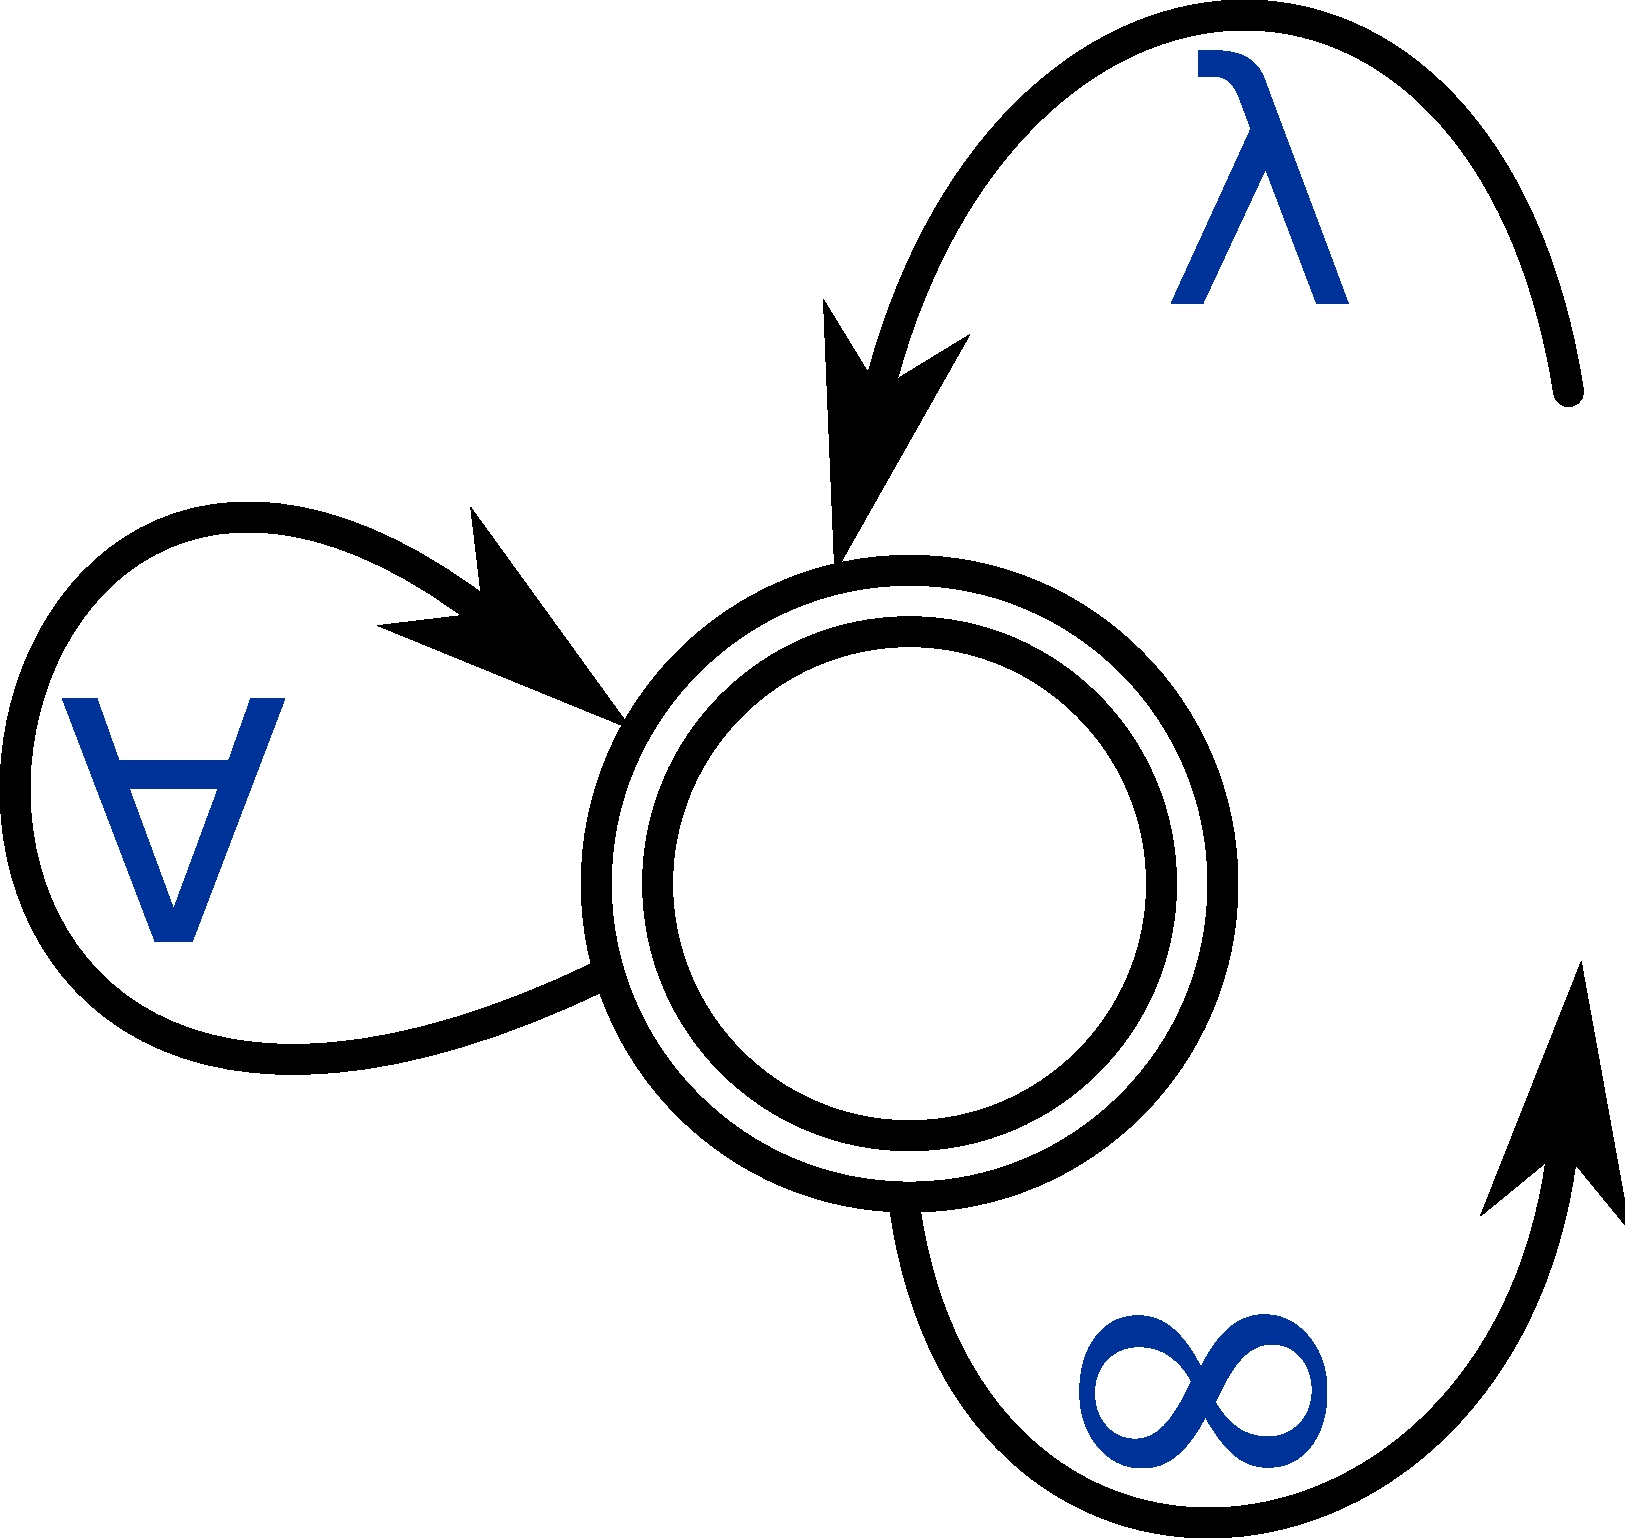
\includegraphics[scale=0.15]{logo.jpg}
	\vspace{2cm}\\
	
	%title
	\Huge \textbf{Argumentation Theory}\\ \large \textbf{Nonmonotonic Reasoning}\\
	\vspace{2cm}
	{\large \textbf{BACHELOR'S THESIS}} \vspace{2.5mm}\\ {\small submitted in partial fulfillment of the requirements for the degree of} \vspace{2.5mm}\\ 
	{\large \textbf{Bachelor of Science}} \vspace{2.5mm}\\ {\small in} \vspace{2.5mm}\\ {\large Software- and Information Engineering} \vspace{2.5mm}\\
	{\small by} \vspace{2.5mm}\\
	%author
	\huge \textbf{Christoph Groß, 1025119}\\
\end{center}
	%advisor
	\vspace{2cm}
\begin{flushleft}
	\begin{adjustwidth}{-0.5in}{}
	{\small to the Faculty of Informatics \\ at the Vienna University of Technology \vspace{2.5mm}\\ Advisor: Ao.Prof.Dipl.-Ing.Dr.techn. Christian Georg Fermüller}
	\end{adjustwidth}
\end{flushleft}

\end{titlepage}
\restoregeometry{}

%Table of Contents
\tableofcontents{}

%Statutory Declaration
\chapter*{Statutory Declaration}
\addcontentsline{toc}{chapter}{Statutory Declaration}

Hereby I assure that this thesis is a result of my personal work and that no other than the indicated aids have been used for its completion.\\
Furthermore I assure that all the quotations and statements, that have been inferred literally or in a general manner from published or unpublished writings, are marked as such.\\
Beyond this I assure that the work has not been used, neither completely nor in parts, to pass any previous examination.

\vspace{1.5cm}
Vienna, \today
\hspace{1.5cm}
\begin{tabular}{l}
\makebox[2.5in]{\hrulefill}\\
Christoph Groß\\
\end{tabular}

%Acknowledgements
\chapter*{Acknowledgements}
\addcontentsline{toc}{chapter}{Acknowledgements}

$D := \{Friends,Family,University\}$\\
$Friends = \{\text{Max,Pia,Lea,Tobi,Johannes}\}$, \\ $Family = \{\text{Sabine,Gerald,Angelika,Johann,Johanna,Patrick}\}$, \\ $University = \{\text{Prof.Fermüller}\}$


%Abstract
\chapter*{Abstract}
\addcontentsline{toc}{chapter}{Abstract}

Throughout this thesis, I am going to explore the applications of argumentation theory in the context of nonmonotonic reasoning.\\
First off, I will introduce the necessary formal definitions, give a few easy examples as clarification and draw the theoretical conclusions.\\
In the next step, the reader is given an overview over the real-life applications of argumentation theory.\\
Finally I will append the documentation of an application specifically written during the course of this thesis, which purpose is to graphically help understanding the subject.\\

\raggedright %left-align whole text
%Chapter 1, Introduction
\chapter{Introduction}

%Nonmonotonic reasoning
\section{Nonmonotonic Reasoning}
When talking about nonmonotonic reasoning, one is referring to the process of deducing knowledge within a formal logic,
whose consequence relation does not fulfill the requirements of monotonicity.

%Definition of Monotonicity :TODO evtl. noch ein bsp. einbauen? auf default logic verweisen?
\begin{elab}[Monotonicity]
If for a given set of formulas $\bm{\psi}$ and a formula $\bm{A}$ the logical consequence $\bm{\psi \vdash A}$ holds,\\ then $\bm{\psi,B \vdash A}$ still holds.
\end{elab}
As one can see, nonmonotonic sets of formulas might change their deducable knowledge as new facts are added. 

\section{Argumentation Theory}
In a human context, we (hopefully) argue to reach a sound conclusion. We do that by claiming statements based on premisses, and usually, due to different perception and other factors,
these statements tend to vary in their degree of believability.

Argumentation Theory, from a logical point of view, tries to formalize these strategies and introduces rules to that purpose. 
Therefore arguments are modeled as formulas which might or might not attack each other.
For instance, the most believeable argument out of two, so to say the "winner", 
would be the one, that attacks the other argument, and at the same time, does not get attacked by said argument.\\
In the following chapter, I will provide all the necessary definitions to achieve the above mentioned aim.
Most of the definitions used in this thesis were originally introduced in \cite{Dung}, some more intuitive forms were found in \cite{Egly}.

\newpage	

\subsection{Argumentation Frameworks}
\begin{mydefn}[Argumentation Framework]
$\bm{AF:=(AR,att)}$
\end{mydefn}

An argumentation framework AF is defined as a tuple, consisting of a set of arguments and a set of attack relations.
The following example should help illustrating this construct a little better.

\begin{myexmpl}
$\bm{s=}$"Superman is the best superhero!", $\bm{b=}$"Batman is way cooler.."\\
$\bm{AR = \{s,b\}}$, $\bm{att=\{(b,s)\}}$
\end{myexmpl}

Since the only tuple in $\bm{att}$ is the one that represents $\bm{b}$ attacking $\bm{s}$, the (frankly obvious) outcome is that $\bm{b}$ is the winning argument.

%Properties of argumentation frameworks
\subsection{Properties of (Sets of) Arguments}

%basic properties: conflict free, acceptable, admissible
\begin{mydefn}[Conflict-freeness]
A set \textbf{S} of arguments is said to be conflict-free, if for any argument $\bm{a \in S}$, there is no other argument $\bm{b \in S}$ so that $\bm{(a,b) \in att}$.
\end{mydefn}

\begin{mydefn}[Acceptability]
An argument $\bm{a \in AR}$ is acceptable with respect to a set \textbf{S}, iff \textbf{S} attacks any argument $\bm{b \in AR}$ that attacks \textbf{a}. 
\end{mydefn}

\begin{myfrmrk}
If for said argument $\bm{a}$ is not being attacked by any $\bm{b \in AR}$, then it is acceptable with even the empty set.
\end{myfrmrk}

\begin{mydefn}[Admissibility]
A conflict-free Set \textbf{S} is said to be admissible, iff each argument $\bm{a \in S}$ is acceptable with respect to \textbf{S}.
\end{mydefn}

These are the basic properties that can be fulfilled by arguments or sets of arguments. Based on them, we will now introduce a few more interesting definitions.
For instance, argumentation theory knows a number of different extensions, which can be used to model the degree of "credulity" of an agent.

Before we discuss those extensions and their implications on argumentation theory, I would like to make a detour and discuss the conventional meaning of extensions in predicate logic.

\newpage

%extensions in prediacte logic
\begin{myelab}[Extensions]
For any n-ary predicate $\bm{\Phi}$, its extension can be written as $\bm{\{(x_{1},...,x_{n})|\Phi(x_{1},...,x_{n})\}}$.\\
So, the extension of a predicate is nothing other than the maximum set of tuples \\ fulfilling said predicate.
\end{myelab}

The aforementioned extensions, adapted fo fit the needs of argumentation theory, use this idea in combination with certain selective criteria to model the desired behaviour. 
The first extension takes a rather gullible approach to things; the so called \textit{preferred extension} is defined as follows:

\begin{myrmrk}
From here on, we will use $E_{i}$ to denote an arbitrary but fixed extension of type $i$, while $E_{I}$ denotes the set of all extensions of type $i$.
\end{myrmrk}

\begin{mydefn}[Preferred Extensions]
$\bm{E_{p}}$ is a preferred extension of \textbf{AF}, iff $\bm{E_{p}}$ is a maximum admissible set of \textbf{AF}.
\end{mydefn}

As you can see, the preferred extension is made up of the biggest, conflict-free set of arguments, that can be defended against all other arguments not in the set.

Another approach would be the \textit{stable extension}, which is defined as follows:
\begin{mydefn}[Stable Extensions]
The conflict-free set $\bm{E_{s}}$ is a stable extension of \textbf{AF}, iff $\bm{E_{s}}$ attacks each argument $\bm{a \notin E_{s}}$; which is equivalent to
$\bm{\{a|a}$ is not attacked by $\bm{E_{s}\}}$.
\end{mydefn}

Apparently, the stable extension contains all arguments that it does not attack itself. Therefore it has to be a conflict-free, admissible set.\\
We will explore the differences between those extensions in a later chapter. 

For now, there are two more types of extensions, which have to be introduced.

\begin{mydefn}[Complete Extensions]
The admissible set $\bm{E_{c}}$ is a complete extension of \textbf{AF}, iff every argument which is acceptable with respect to $\bm{E_{c}}$, is included in $\bm{E_{c}}$.
\end{mydefn}

It is easy to see that many different complete extensions can exist, depending on $E_{c}$. That leads directly to the \textit{grounded extension}.

\begin{mydefn}[Grounded Extensions]
The intersection of all complete extensions is called the grounded extension. $\bm{E_{g} := \bigcap{comp(AF)}}$
\end{mydefn}

Since all the necessary, basic definitions of argumentation frameworks have been laid out, I will go on and provide the promised examples.

\newpage

\subsection{Examples of different Extensions}
By expanding example 1.1 with a few more arguments, we now have to consider the following example.

\begin{myexmpl}
$\bm{s_{1}=}$"Superman is the best superhero!", $\bm{b_{1}=}$"Batman is way cooler..",\\
$\bm{s_{2}=}$"But Superman is stronger.", $\bm{b_{2}=}$"Batman possesses genius-level intellect."\\
$\bm{AR = \{s_{1},s_{2},b_{1},b_{2}\}}$, $\bm{att = \{(b_{1},s_{1}),(s_{2},b_{1}),(b_{2},s_{2})\}}$
\label{s1 s2 b1 b2 ex}
\end{myexmpl}

This argumentation framework could also be depicted by following graph.

\begin{figure}[h!]
\begin{center}\begin{tikzpicture}
	\node[state](s1){$s_{1}$};
	\node[state](b1)[right=of s1]{$b_{1}$};
	\node[state](s2)[right=of b1]{$s_{2}$};
	\node[state](b2)[right=of s2]{$b_{2}$};
	\path[->,thick] (b2) edge (s2);
	\path[->,thick] (s2) edge (b1);
	\path[->,thick] (b1) edge (s1);
\end{tikzpicture}\end{center}
\caption{graph of AF (example \ref{s1 s2 b1 b2 ex})}
\end{figure}

The extensions of this example would be 
\begin{itemize}
	\item{$\bm{E_{P}=E_{S}=E_{C}=E_{G}=\{\{b_{1},b_{2}\}\}}$}
\end{itemize}

\bigskip
The next example is going to be a little more interesting in its outcome.
\begin{myexmpl}
$\bm{s=}$"Superman was born a hero.", $\bm{b=}$"Batman trained hard to become a hero."\\
$\bm{AR=\{s,b\}}$, $\bm{att=\{(s,b),(b,s)\}}$
\label{s b ex}
\end{myexmpl}

This examples graph looks like this.
\begin{figure}[h!]
\begin{center}\begin{tikzpicture}
	\node[state](s){$s$};
	\node[state](b)[right=of s]{$b$};
	\path[->,thick](s) edge[bend left] (b);
	\path[->,thick](b) edge[bend left] (s);
\end{tikzpicture}\end{center}
\caption{graph of AF (example \ref{s b ex})}
\end{figure}

Following extensions can be calculated
\begin{itemize}
	\item{$\bm{E_{P}=E_{S}=\{\{s\},\{b\}\}}$}
	\item{$\bm{E_{C}=\{\{\emptyset\},\{s\},\{b\}\}}$}
	\item{$\bm{E_{G}=\{\{\emptyset\}\}}$}
\end{itemize}

\newpage

The following example (on the contrary to the above) has different preferred and stable extensions.

\begin{myexmpl}
$\bm{b=}$"Batman is Clark Kent."\\
$\bm{AR=\{b\}}$, $\bm{att=\{(b,b)\}}$
\label{b loop ex}
\end{myexmpl}

The corresponding graph looks like follows.
\begin{figure}[h!]
\begin{center}\begin{tikzpicture}
	\node[state](b){$b$};
	\path[->,thick](b) edge[loop left] (b);
\end{tikzpicture}\end{center}
\caption{graph of AF (example \ref{b loop ex})}
\end{figure}

For this last example here, the extensions would look as follows.
\begin{itemize}
	\item{$\bm{E_{P}=E_{C}=E_{G}=\{\{\emptyset\}\}}$}
	\item{$\bm{E_{S}=\{\emptyset\}}$}
\end{itemize}

\chapter{Conclusions and Implications}

Now that we have established the basic definitions, it is time to travel further down the rabbit hole and explore the meaning of what we just defined.

\section{Relations between different Extensions}
First off, I want to clarify a few relations between those aforementioned extensions, since they can be reused in later proofs.

\begin{mylem}
%latex interprets the first item of the list as a sentence, therefore this "bogus" first sentence.
\leavevmode\vspace{-\baselineskip}
\begin{enumerate}
	\item{Every preferred extension is a complete extension, but not vice versa.}
	\item{The ground extension is the least (with respect to set inclusion) complete extension}
\end{enumerate}
\end{mylem}

\begin{myprf}[1]
It is obvious that every preferred extension (maximum admissible set) is a complete extension. So we only need to show that the other way round is not true.

Assumption: Every complete extension is also a preferred extension.\\
Let $\bm{AR=\{a,b\}}$ and $\bm{att=\{(a,b),(b,a)\}}$.\\
Then it is easy to see, that $\bm{E_{P}=\{\{a\},\{b\}\}}$ but $\bm{E_{C}=\{\emptyset,\{a\},\{b\}\}}$\\
$\bm{\implies \exists E_{c}: E_{c} \in E_{C} \land E_{c} \notin E_{P} \implies \text{\Lightning}}$
\end{myprf}

\begin{myprf}[2]
Proof for this lemma follows directly from the definition of ground extensions.
\end{myprf}

\newpage

\section{Properties of Argumentation Frameworks}
Up to now, we have only talked about sets of arguments and their properties. Now we will take a closer look at the whole argumentation framework and 
make a connection between its properties and extensions.

\subsection{Well-Founded Argumentation Frameworks}
The first new property establishes a coherence between preferred, grounded and stable extensions.
\begin{mydefn}[Well-Founded Argumentation Frameworks]
An argumentation framework is considered well-founded, iff there exists no infinit sequence of arguments $A_{0},A_{1},...,A_{n},...$ where each $A_{i+1}$ attacks $A_{i}$.
\end{mydefn}

\begin{myfrmrk}
This infinite sequence of arguments can be formed by a finite set of arguments (for instance $AR=\{a,b\}$, $att={(a,b),(b,a)}$).
\end{myfrmrk}

Although it might not be the most intuitive observation, following lemma can be extracted from this definition.
\begin{mylem}
Every well-founded AF has exactly one complete extension, which is also a preferred, grounded and stable extension.
\end{mylem}

\begin{myprf}
Assumption: $\bm{\exists AF: \text{AF is well-founded and } E_{p}=E_{c}=E_{g} \notin E_{S}}$.
We further assume, that $\bm{\exists a \in AR \text{\textbackslash} E_{g} \text{ and } \nexists b \in E_{g}:(b,a) \in att}$.\\
\bigskip
If $\bm{a}$ is not acceptable with respect to $\bm{E_{g}}$, this means that there has to be another argument $\bm{c \in AR \text{\textbackslash} E_{g}}$, 
which is also not attacked by $\bm{E_{g}}$. \\ Therefore an infinite sequence of arguments like $\bm{a \text{ and }c}$ has to exist $\implies \text{\Lightning}$.
\end{myprf}

\subsection{Coherent Argumentation Frameworks}


















%Bibliography - references to papers
\begin{thebibliography}{1}
	\bibitem[\textbf{Dung}]{Dung} "On the acceptability of arguments and its fundamental role in nonmonotonic reasoning,...";\\Phan Minh Dung; 1995
	\bibitem[\textbf{EgGaWo}]{Egly} "Answer-Set Programming Encodings for Argumentation Frameworks"; Uwe Egly, Alice Gaggl, Stefan Woltran; 2010  
\end{thebibliography}

\end{document}
